\documentclass[a4paper,12pt]{article}
\usepackage{graphicx}
\usepackage{amsmath, amssymb}
\usepackage{float}
\usepackage{subcaption}
\usepackage{siunitx}
\usepackage{hyperref}
\usepackage{circuitikz}

\title{\textbf{Op-Amp Applications}}
\author{Sai Akhila-EE24BTECH11055 \\Sai Akshita-EE24BTECH11054}
\date{\today}

\begin{document}

\maketitle

\section{Objective}
\begin{itemize}
    \item Implementing a custom weighted summing and difference amplifier.
    \item Implementing an Op-amp integrator.
    \item Rectification of AC signals without the voltage drop issue of a diode.
\end{itemize}

\section{Structure and Working of Op-Amp}
\begin{figure}[H]
    \centering
    \includegraphics[width=0.8\textwidth]{fig/o.jpeg} % Adjust width as needed
    \caption{Op-Amp design}
    \label{fig:image_label}
\end{figure}
\begin{figure}[H]
    \centering
	\includegraphics[width=0.8\textwidth]{fig/p.jpeg} % Adjust width as needed
    \caption{Op-Amp design}
    \label{fig:image_label}
\end{figure}
$V_{cc}$ : This pin is the positive voltage supply to the Op-Amp.

\section{Custom weighted summing and difference amplifier}

\subsection{Materials Required}
\begin{itemize}
    \item Op-Amp(LM$358$)-2
    \item Resistors(10k$\Omega$)-9
    \item DC power supply
    \item Function Generator
    \item Oscilloscope
    \item Jumper wires
\end{itemize}
\subsection{Circuit Design}
\begin{itemize}
    \item Connect the Op-Amps and resistors as shown in the figure below. 
    \item Give $V_{cc}$ a positive input and GND a negative voltage.
    \item Give voltage input for $V_1$, $V_2$ and $V_3$ from the DC power supply and Function Generator.
    \item Measure the output voltage at the output pin of the third Op-Amp using the oscilloscope probe. 
\end{itemize}
\subsection{Circuit Diagram}
\begin{figure}[H]
\centering
\resizebox{1.1\textwidth}{!}{%
\begin{circuitikz}
\tikzstyle{every node}=[font=\LARGE]
\draw [ line width=0.8pt](4,9.5) to[american voltage source,l={ \normalsize V1}] (4,7.25);
\draw [ line width=0.8pt](5.25,4.5) to[american voltage source,l={ \normalsize V2}] (5.25,3.25);
\draw [ line width=0.8pt](6.5,0.5) to[american voltage source,l={ \normalsize V3}] (6.5,-0.75);
\draw [ line width=0.8pt](5,9.5) to[R,l={ \normalsize R}] (7,9.5);
\draw [ line width=0.8pt](7,4.75) to[R,l={ \normalsize R}] (9,4.75);
\draw [ line width=0.8pt](9.25,0.75) to[R,l={ \normalsize R}] (11.25,0.75);
\draw [ line width=0.8pt](11.25,6.25) to[R,l={ \normalsize R}] (13.25,6.25);
\draw [ line width=0.8pt](10.75,11.25) to[R,l={ \normalsize 2R}] (12.75,11.25);
\draw [ line width=0.8pt](17,9.75) to[R,l={ \normalsize R}] (19,9.75);
\draw [ line width=0.8pt](18.5,4.75) to[R,l={ \normalsize R}] (20.5,4.75);
\draw [ line width=0.8pt](23.5,7.75) to[R,l={ \normalsize R}] (25.5,7.75);
\draw [ line width=0.8pt](4,9.5) to[short] (5,9.5);
\draw [ line width=0.8pt](7,4.75) to[short] (5.25,4.75);
\draw [ line width=0.8pt](5.25,4.5) to[short] (5.25,5);
\draw [ line width=0.8pt](9.25,0.75) to[short] (6.5,0.75);
\draw [ line width=0.8pt](6.5,0.5) to[short] (6.5,1);
\draw [ line width=0.8pt](13.25,3.5) node[op amp,scale=1, yscale=-1 ] (opamp2) {};
\draw [ line width=0.8pt](opamp2.+) to[short] (11.75,4);
\draw [ line width=0.8pt] (opamp2.-) to[short] (11.75,3);
\draw [ line width=0.8pt](14.45,3.5) to[short](14.75,3.5);
\draw [ line width=0.8pt](25.25,4.25) node[op amp,scale=1, yscale=-1 ] (opamp2) {};
\draw [ line width=0.8pt](opamp2.+) to[short] (23.75,4.75);
\draw [ line width=0.8pt] (opamp2.-) to[short] (23.75,3.75);
\draw [ line width=0.8pt](26.45,4.25) to[short](26.75,4.25);
\draw (12.5,8.75) node[op amp,scale=1, yscale=-1 ] (opamp2) {};
\draw (opamp2.+) to[short] (11,9.25);
\draw  (opamp2.-) to[short] (11,8.25);
\draw (13.7,8.75) to[short](14,8.75);
\draw [ line width=0.8pt](7,9.5) to[short] (7,8.25);
\draw [ line width=0.8pt](11,8.25) to[short] (7,8.25);
\draw [ line width=0.8pt](10.75,11.25) to[short] (10.75,8.25);
\draw [ line width=0.8pt](12.75,11.25) to[short] (13.5,11.25);
\draw [ line width=0.8pt](13.5,11.25) to[short] (13.5,8.75);
\draw [line width=0.8pt](11,9.25) to (11,9) node[ground]{};
\draw [line width=0.8pt](11.75,4) to (11.75,3.75) node[ground]{};
\draw [line width=0.8pt](23.75,4.75) to (23.75,4.5) node[ground]{};
\draw [ line width=0.8pt](9,4.75) to[short] (9,2.75);
\draw [ line width=0.8pt](11.75,3) to[short] (9,3);
\draw [ line width=0.8pt](11.25,6.25) to[short] (10.5,6.25);
\draw [ line width=0.8pt](10.5,6.25) to[short] (10.5,3);
\draw [ line width=0.8pt](13.25,6.25) to[short] (14.5,6.25);
\draw [ line width=0.8pt](14.5,6.25) to[short] (14.5,3.5);
\draw [ line width=0.8pt](14.75,3.5) to[short] (18.5,3.5);
\draw [ line width=0.8pt](18.5,4.75) to[short] (18.5,3.5);
\draw [ line width=0.8pt](13.75,8.75) to[short] (17,8.75);
\draw [ line width=0.8pt](17,9.75) to[short] (17,8.75);
\draw [ line width=0.8pt](11.25,0.75) to[short] (21.75,0.75);
\draw [ line width=0.8pt](19,9.75) to[short] (22,6.75);
\draw [ line width=0.8pt](20.5,4.75) to[short] (22.25,6.5);
\draw [ line width=0.8pt](21.5,7.25) to[short] (22.25,6.5);
\draw [ line width=0.8pt](21.75,0.75) to[short] (22.25,0.75);
\draw [ line width=0.8pt](22.25,6.5) to[short] (22.25,0.75);
\draw [ line width=0.8pt](23.75,3.75) to[short] (22.25,3.75);
\draw [ line width=0.8pt](23.5,7.75) to[short] (22.5,7.75);
\draw [ line width=0.8pt](22.5,7.75) to[short] (22.5,3.75);
\draw [ line width=0.8pt](25.5,7.75) to[short] (27,7.75);
\draw [ line width=0.8pt](27,7.75) to[short] (27,4.25);
\draw [ line width=0.8pt](26.5,4.25) to[short] (27.5,4.25);
\draw [ line width=0.8pt](27.5,4.25) to[short] (29.5,4.25);
\draw [line width=0.8pt, ->, >=Stealth] (14.25,9) -- (16.25,9);
\draw [line width=0.8pt, ->, >=Stealth] (15.5,3.75) -- (17.5,3.75);
\draw [line width=0.8pt, ->, >=Stealth] (15,1) -- (17,1);
\draw [line width=0.8pt, ->, >=Stealth] (23.5,8.75) -- (25.5,8.75);
\node [font=\LARGE] at (15.5,9.5) {-2V1/R};
\node [font=\LARGE] at (16.5,4.25) {-V2/R};
\node [font=\LARGE] at (16,1.5) {V3/R};
\node [font=\LARGE] at (24.25,9.25) {-2V1/R-V2/R+V3/R};
\node [font=\LARGE] at (29,3.25) {Vo = 2V1+V2-V3};
\draw [ line width=0.8pt](27.75,4.25) to[short, -o] (29.75,4.25) ;
\draw [ line width=0.8pt](29.75,0.25) to[short, -o] (29.75,2.5) ;
\draw [line width=0.8pt](4,7.25) to (6,7.25) node[ground]{};
\draw [line width=0.8pt](5.25,3.25) to (7.25,3.25) node[ground]{};
\draw [line width=0.8pt](6.5,-0.75) to (8.5,-0.75) node[ground]{};
\draw [line width=0.8pt](29.75,0.25) to (31.75,0.25) node[ground]{};
\draw [line width=0.8pt, ->, >=Stealth] (4.75,10.75) -- (6.75,10.75);
\draw [line width=0.8pt, ->, >=Stealth] (5.25,5.25) -- (7.5,5.25);
\node [font=\LARGE] at (5.5,11.25) {V1/R};
\node [font=\LARGE] at (6,5.75) {V2/R};
\end{circuitikz}
}%

\label{R1}
\end{figure}
\begin{figure}[H]
    \centering
    \includegraphics[width=0.8\textwidth]{fig/c1.jpeg} % Adjust width as needed
    \caption{Caption describing the image}
    \label{fig:image_label}
\end{figure}
\subsection{Working Principle}
The given circuit consists of two inverting op-amps used to modify voltage signs and a summation amplifier to combine the signals. The circuit operates as follows:

\begin{enumerate}
    \item \textbf{First Inverting Op-Amp}  
    \begin{itemize}
        \item The first operational amplifier (Op-amp) is configured as an inverting amplifier with a gain of $-2$.
        \item It takes the input voltage $V_1$ and produces an output of $-2V_1$.
    \end{itemize}
    
    \item \textbf{Second Inverting Op-Amp}  
    \begin{itemize}
        \item The second op-amp is also an inverting amplifier but with a gain of $-1$.
        \item It inverts the input voltage $V_2$, giving an output of $-V_2$.
    \end{itemize}
    
    \item \textbf{Summing Amplifier}  
    \begin{itemize}
        \item The outputs of the first and second inverting amplifiers, along with $V_3$, are fed into a \textbf{summing amplifier}.
        \item The summing amplifier performs a weighted addition of the inputs:
        \[
        V_o = 2V_1 + V_2 - V_3
        \]
        \item This means the final output voltage is a combination of the amplified and inverted signals from the previous stages.
    \end{itemize}
\end{enumerate}

\subsection{Observations}
In our case, 
$$V_{1}=5, 
V_2=3, 
V_3=5$$
$$V_{cc}=12 V, GND = -12 V$$
\begin{figure}
    \centering
    \includegraphics[width=0.5\linewidth]{fig/8v.jpeg}
    \caption{Output Voltage-1}
    \label{fig:enter-label}
\end{figure}
Thus we get our output voltages as:\\
\begin{itemize}
    \item $V_0=2V_1+V_2-V_3=2(5)+3-5=8V$\\
    \item $V_0=2V_1-V_3=5V$
\end{itemize}
\begin{figure}
    \centering
    \includegraphics[width=0.5\linewidth]{fig/5v.jpeg}
    \caption{Output Voltage-2}
    \label{fig:enter-label}
\end{figure}
\subsection{Precautions}
\begin{enumerate}
    \item Ensure all the connections are firm and tight.
    \item Ensure that the resistors don't touch each other.
    \item Ensure that the resistors don't touch the Op-amp pins.
    \item Check the data sheet for the Op-amp being used for the maximum and minimum inputs it can handle.
\end{enumerate}
\section{ Op-amp integrator}

\subsection{Materials Required}
\begin{itemize}
     \item Op-Amp (LM-$358$)
    \item Resistors (10 k$\Omega$, 100 k$\Omega$)
    \item Capacitor ($220$ nF)
    \item Function Generator
    \item Oscilloscope
    \item Jumper wires
\end{itemize}

\subsection{Circuit Diagram}
\begin{figure}[H]
\centering
\resizebox{1.1\textwidth}{!}{%
\begin{circuitikz}
\tikzstyle{every node}=[font=\LARGE]

\draw [ line width=0.8pt](20,5.5) node[op amp,scale=1, yscale=-1 ] (opamp2) {};
\draw [ line width=0.8pt](opamp2.+) to[short] (18.5,6);
\draw [ line width=0.8pt] (opamp2.-) to[short] (18.5,5);
\draw [ line width=0.8pt](21.2,5.5) to[short](21.5,5.5);
\draw [ line width=0.8pt](18.5,5) to[short] (16.5,5);
\draw [ line width=0.8pt](16.5,5) to[short] (16.5,7.75);
\draw [ line width=0.8pt](16.5,7.75) to[short] (18,7.75);
\draw [line width=0.8pt](18,7.75) to[C,l={ \LARGE C}] (21.75,7.75);
\draw [ line width=0.8pt](21.75,7.75) to[short] (21.75,5.5);
\draw [ line width=0.8pt](21.5,5.5) to[short] (22.75,5.5);
\draw [ line width=0.8pt](22.75,5.5) to[short, -o] (22.75,4.5) ;
\draw [ line width=0.8pt](22.75,2.5) to[short, -o] (22.75,3.75) ;
\draw [line width=0.8pt](22.75,2.5) to (24.75,2.5) node[ground]{};
\draw [line width=0.8pt](18.5,6) to (17.75,6) node[ground]{};
\draw [ line width=0.8pt](16.5,5) to[R,l={ \LARGE R}] (14.25,5);
\draw [ line width=0.8pt](14.25,5) to[american voltage source] (14.25,3.75);
\draw [line width=0.8pt](14.25,3.75) to (16.25,3.75) node[ground]{};
\node [font=\LARGE] at (13.5,4.25) {V};
\node [font=\LARGE] at (23.5,4) {Vo};
\node [font=\LARGE] at (23.5,5) {+};
\node [font=\LARGE] at (23.5,3.25) {-};
\draw [line width=0.8pt, ->, >=Stealth] (14.5,5.75) -- (16,5.75);
\node [font=\LARGE] at (15.25,6.25) {V/R};
\end{circuitikz}
}%

\label{R1}
\end{figure}

\begin{figure}
    \centering
    \includegraphics[width=0.5\linewidth]{fig/c2.jpeg}
    \caption{Circuit-Integrator}
    \label{fig:enter-label}
\end{figure}

\subsection{Working Principle}
An operational amplifier (op-amp) integrator is a circuit that performs mathematical integration of the input voltage with respect to time. \\The circuit consists of an op-amp with a capacitor in the feedback path and a resistor at the input. 
\begin{enumerate}
   
    \item \textbf{Capacitor Charging and Feedback}
    \begin{itemize}
        \item Since the op-amp maintains virtual ground, the current through $R$ is given by Ohm’s law:
        \[
        I = \frac{V_{in}}{R}
        \]
        \item This current cannot flow into the op-amp’s input and is forced to flow through the feedback capacitor $C$.
        \item The voltage across a capacitor is given by:
        \[
        V_C = \frac{1}{C} \int I \, dt
        \]
        \item Substituting $I = \frac{V_{in}}{R}$:
        \[
        V_o = - \frac{1}{RC} \int V_{in} \, dt
        \]
    \end{itemize}

   
\end{enumerate}
\subsection{Observations}
 The output voltage $V_o$ is the negative integral of the input voltage.
 Since the input is a square wave, we get the output wave as a trangular wave.
\begin{figure}[H]
    \centering
    \includegraphics[width=0.7\textwidth]{fig/rc.jpeg} % Replace with actual file
    \caption{Output signal}
\end{figure}

\section{ Precision Rectifier}

\subsection{Materials Required}
\begin{itemize}
    \item 2 Op-Amps (LM-358)
    \item 2 diodes (1N4148)
    \item Breadboard
    \item Connecting wires
    \item Resistors of $10k\Omega$-5
    \item AC power supply
    \item Oscilloscope with probes
\end{itemize}


\subsection{Circuit Diagram}
\begin{figure}[H]
    \centering
    \includegraphics[width=0.7\textwidth]{fig/hf.jpeg} % Replace with actual file
    \caption{Half-wave and Full-wave rectifier}
\end{figure}

\subsection{Working Principle}
\textbf{Half-Wave Precision Rectifier:}\\
This circuit consists of 2 diodes and a single Op-Amp. When the signal's at a certain time between 0 to $\frac{T}{2}$, the current passes through the circuit as shown in the following picture, due to the fact that the diodes are forward biased in this situation.\\

When the signal's at a certain time between $\frac{T}{2}$ to $T$[insert mage], the current flows through the feedback resistor path, and thus the Op-Amp inverts the negative voltage and gives off positive voltage as the output.\\
Hence only the part of the sine wave that has negative amplitude, ranging from 0 to 2 volts is inverted and passed and recorded by the oscilloscope as shown in the figure (observation).\\
\textbf{Full-Wave Precision Rectifier:}\\
For the circuit used for Full-Wave Rectification, the diodes in Half-Wave Rectifier circuit are reversed followed by giving both $V_1$ and $V_o$ of half wave rectifier to the $V^-$ pin of another Op-Amp.\\\\ One important thing to note is that in this circuit between $V_o$ of sub-circuit and $v^-$ pin of 2nd Op-Amp, a resistance of $5k\Omega$ is connected by putting 2 $10k\Omega$ in parallel connection.\\
From the point, P2 to point P3 is the summing amplifier, the output from the precision rectifier is fed to the summing amplifier through the resistor R3. The value of the resistor R3 is half of R5 or you can say it’s R5/2=$5k\Omega$ that is how we are setting a 2X gain out of the op-amp.\\
The input from the point P1 is also fed to the summing amplifier with the help of the resistor R4, the resistors R4 and R5 are responsible for setting the gain of the op-amp to 1X.\\
Since the output from the Point P2 is fed directly to the summing amplifier with the gain of 2X, that means the output voltage will be 2-times the input voltage. Let's assume the input voltage is 2V peak, so we will get a 4V peak at the output. At the same time, we are directly feeding the input to the summing amplifier with a gain of 1X.
[insert image]
This working principle ensures that the entire sinusoidal wave is rectified. 


\subsection{Observations}
\textbf{Half-wave rectifier:}
\begin{figure}[H]
    \centering
    \includegraphics[width=0.7\textwidth]{fig/h.jpeg} % Replace with actual file
    \caption{Half-wave rectified response of sinusoidal wave}
\end{figure}
\textbf{Full-wave rectifier:}
\begin{figure}[H]
    \centering
    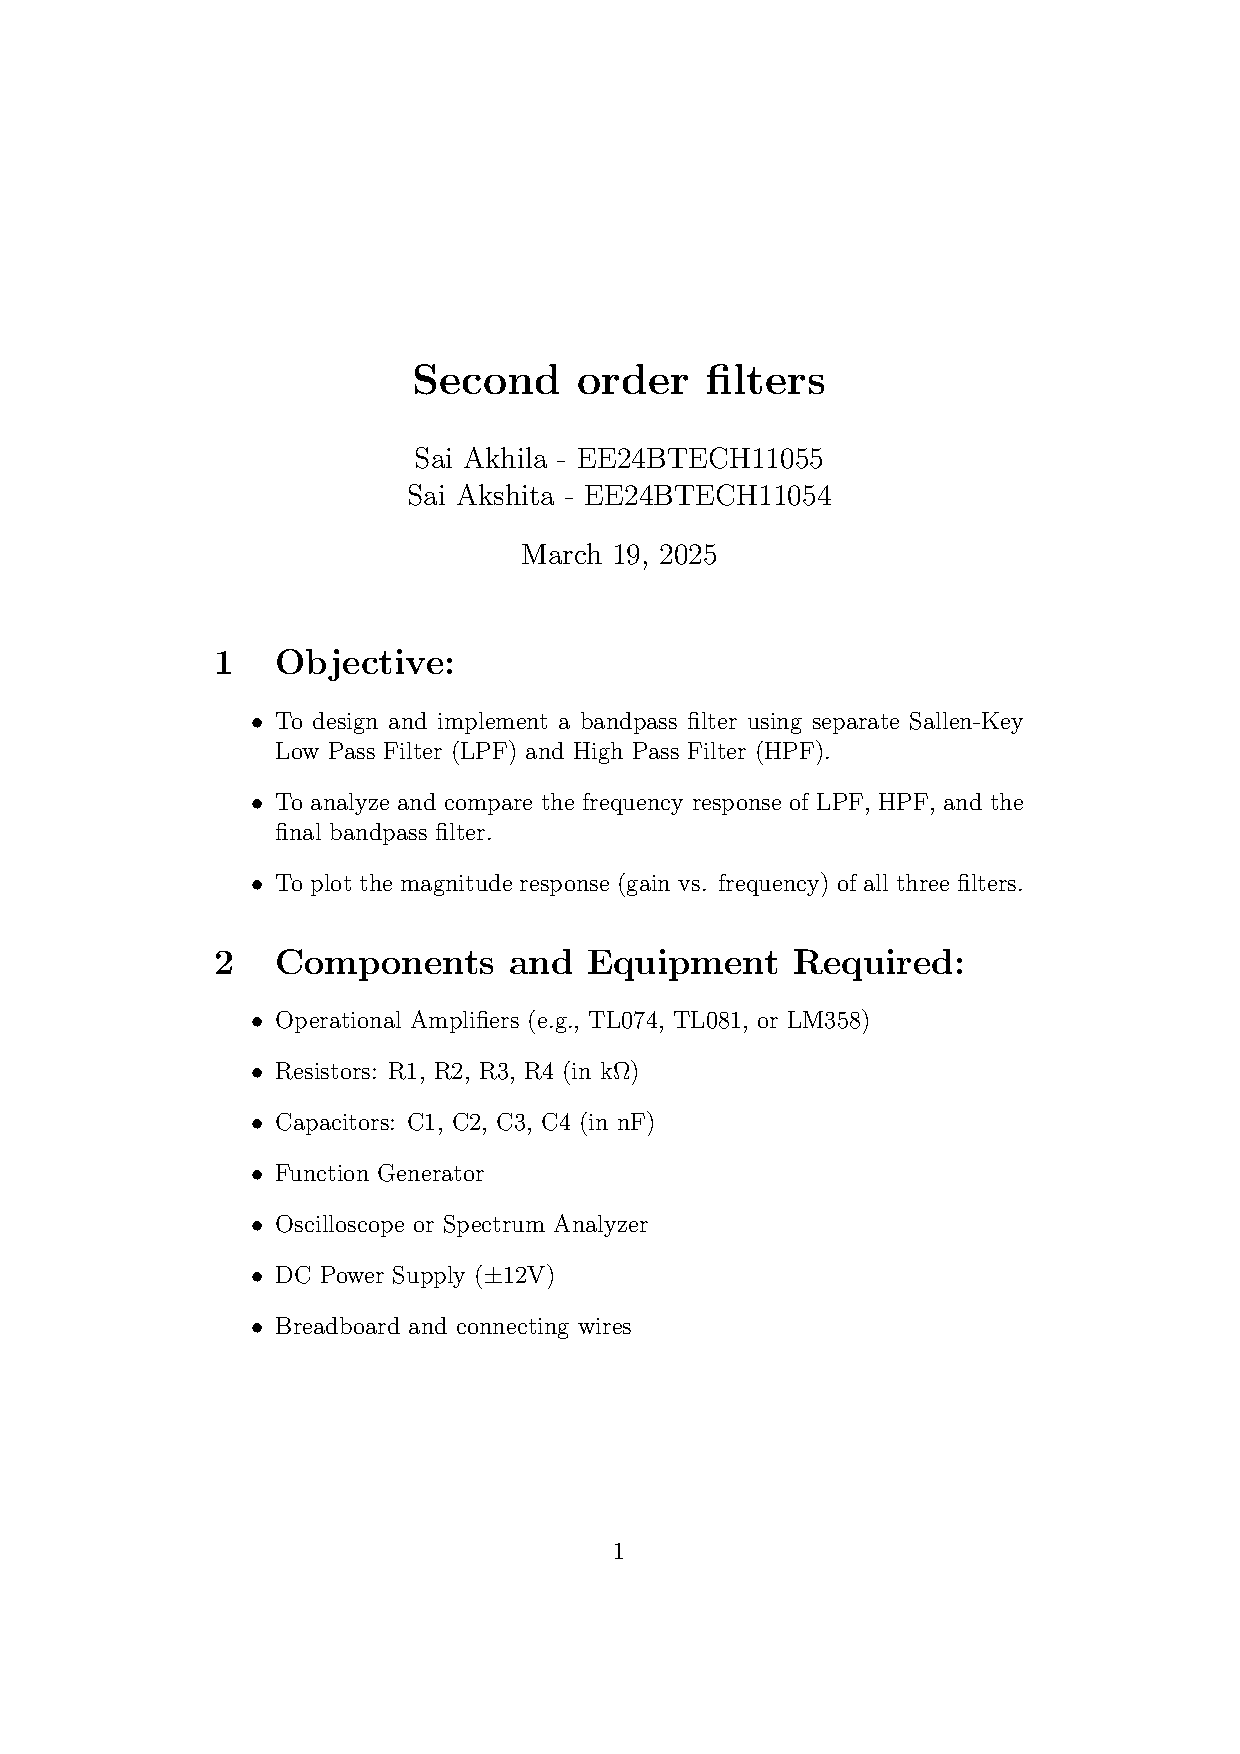
\includegraphics[width=0.7\textwidth]{fig/f.jpeg} % Replace with actual file
    \caption{Full-wave rectified response of sinusoidal wave}
\end{figure}
\subsection{Precautions}
\begin{enumerate}
    \item Ensure that all the connections are strong and tight.
    \item Ensure that the resistors do not touch each other.
    \item Ensure that Op-Amp and diodes are functioning properly.
\end{enumerate}

\section{Final Conclusion}
By performing Experiment-5, we understood the functionality of Op-Amps and diodes. We also understood the principle behind implementing a custom weighted summing and difference amplifier, implementing an Op-Amp integrator, and rectification of AC signals without the voltage drop issue of a diode.

\end{document}
